\documentclass[11pt, letter]{article}

% Load packages
\usepackage[style = authoryear, autocite=inline, doi=false,isbn=false,url=false]{biblatex}
\usepackage[margin = 1 in]{geometry}
\usepackage[colorlinks, citecolor = red]{hyperref}
\usepackage{amsmath, amssymb} %essential
\usepackage[long, nodayofweek]{datetime}
\usepackage[]{booktabs}
\usepackage{graphicx}
\usepackage{setspace}
\usepackage{todonotes}

% For sans-serif (\sffamily) captions and headings:
	\usepackage[sf,pagestyles]{titlesec} % make section headings \sffamily
	% make headers \sffamily
	\newpagestyle{main}[\sffamily]{
	    \sethead{\thepage}{}{\sectiontitle}
	    }
	\pagestyle{main}
	\usepackage{titling}
	% make titling elements \sffamily
	\pretitle{\begin{center}\sffamily\LARGE}
	\preauthor{\begin{center}
	            \large\sffamily \lineskip 0.5em%
	            \begin{tabular}[t]{c}}
	\predate{\begin{center}\sffamily\large}
	\usepackage{abstract}
	% make abstract title \sffamily
	\renewcommand\abstractnamefont{\sffamily}
	\usepackage{caption} 
	\captionsetup{font=sf, labelfont = bf}

% Define symbols
\DeclareRobustCommand{\bbone}{\text{\usefont{U}{bbold}{m}{n}1}}
\DeclareMathOperator{\EX}{\mathbb{E}} % expected value
\DeclareMathOperator{\V}{\mathbb{V}}
\DeclareMathOperator{\Prob}{\mathbb{P}}

\begin{document}
\author{Andrew C. Eggers\thanks{Nuffield College and Department of Politics and International Relations, University of Oxford, United Kingdom. \texttt{aeggers@nuffield.ox.ac.uk}}
\and
Tobias Nowacki\thanks{Department of Political Science, Stanford University, CA, United States. \texttt{tnowacki@stanford.edu}}}
\date{\today}
\title{Strategic Voting under Ranked Choice Voting and Plurality: Empirics}

\maketitle

\doublespacing % set line space

\listoftodos

\section{Link to previous sections / Intro to Empirics}

Up to this point, we have achieved the following: we pointed out why thinking about strategic voting is important (Section 1); we explained our general approach to calculating strategic vote incentives (Section 2); we explained strategic vote incentives under different electoral systems (Plurality and RCV) and derived predictions for the most likely types of strategic incentive conditional on the ``class'' of the ballot profile. The theoretical approach illuminates the mechanics behind the strategic incentives and is useful for understanding where the motivation for insincere ballot orderings originates. 

(Theory $\rightarrow$ Empirics)

However, in order to achieve this, we necessarily assumed ``ideal cases'' in order to reduce complexity and facilitate the theoretical analysis. As set out in Section 3, the distribution of strategic incentives depends on a number of parameters: the full ballot profile -- that is, the distribution of both first \emph{and} second preferences -- the level of information, $s$, the distribution of preferences and their intensity. Jointly, there are too many permutations of these inputs to be able to make meaningful and accurate predictions for each instance. One way of dealing with this issue would be to hold all parameters at mean or representative values and examine the comparative statics of each parameter in turn. (This may work for parameters where we have monotonic predictions, e.g., $s$.) However, doing so would still leave us with manyfold dimensions; furthermore, this approach brushes over the important issue of interaction effects. This is particularly relevant when it comes to describing ballot profiles, where the effects of a change in $A$'s vote will strongly depend on how the remainder is split up between $B$ and $C$, and how second preferences are distributed.

We therefore decided to restrict our empirical analysis to three objectives. First, we want to see whether the classification of ballot profiles according to second preferences ($A+$, $B+$, etc.) can be a helpful predictor of what kind of strategic incentives we can expect in this situation.\footnote{Our highly stylised classes made assumptions about what other pivotal events are likely / unlikely. We don't have any prior on whether these are holding up in the empirics?} We find that, despite significant variance in pivotal probabilities within each class, the predictions for the most dominant type of strategic voting hold. Second, given the distribution of likely ballot profiles (and thus beliefs), we want to compare the overall distribution of strategic incentives (their prevalence and magnitude) under both plurality and RCV. We find that RCV offers more common incentives to vote strategically, but that these incentives are smaller in terms of magnitude, that is $\tau$. Lastly, we compare the overall performance of the two electoral systems: which one is more likely to suffer from a voting paradox, and which one benefits the Condorcet winner more? We find that RCV performs better in both categories: fewer paradoxes, and more helpful to the Condorcet winner. Before we present our analysis of these three questions, we shall briefly discuss our methodology and summarise the CSES data set.

% \subsection{Justification for using CSES data}

% \emph{Maybe scrap this section since approach explained in Section 2?}

% \todo[inline]{Re-work justification so that it fits with the introduction above.}
% We have a general idea that these things should hold true in our idealised cases that we discussed in the theory; but a lot will depend on whether the empirical cases conform to the idealised world, or whether they are outlying and extreme. (There are also some aspects of our theory that yielded ambiguous predictions, which we need to evaluate.)

% How can we test this in practice? The ideal research design would have us run multiple elections -- each with voters who have different beliefs about the likely outcome, and different preferences -- and run these elections twice: once under RCV, and once under Plurality.

% Of course, this is not feasible. A major obstacle is that we do not have a data set that matches voters sincere preferences with their actual voting behaviour. We get close to that in surveys under the assumption that the reported answers are true. But here, we only record the vote choice under the \textit{actual} electoral system -- which, in the vast majority of cases -- is just Plurality. Even in cases where the electoral system in question is RCV, such as Australia, respondents are at most asked about their top two preferences; furthermore, evidence suggests that respondents' recorded answers about rankings past second are inaccurate.

% Thus, we are faced with a significant limitation: we cannot observe whether voters truly cast votes in a strategic fashion or not. Instead, we focus on voters' (presumptively) true preferences, and on simply examining the \textit{incentive} to vote strategically. (We're not interested, at least for now, whether they actually follow that incentive or not). To that end, we take the CSES, a collection of 160 surveys from XX countries before major legislative elections, as our main source for empirical analysis. For each of the cases contained within, we take the sample of voters as representative of the electorate. We assume that they were just given a poll result (forecast) of that election that corresponds to the CSES case sample, where everyone votes according to their sincere preferences. For each voter within that sample, we then calculate their strategic voting incentive: what ballot ordering is optimal, conditional on the beliefs about the outcome and everyone else voting sincerely? (We look at what happens when voters assume that others may vote strategically, too, in Subsection~\ref{interdep}.)

\section{Data and Method}

Our objective in this paper is to measure strategic \emph{incentives}, not actual behaviour. In an ideal setting, we would have access to a dataset that contains information on both voters' sincere preferences and their observed vote choice under different electoral systems. Unfortunately, such a rich data set does not exist.\footnote{Even worse, even in countries with RCV as their main legislative electoral system, survey respondents are typically not asked about their ballot ranking beyond their first or second preferences. XXXX demonstrates that, even if they were, responses are likely to be inaccurate.} Instead, we focus the CSES data, which contains pre-election voter surveys from 160 cases. In each case, respondents (who are weighted such that the survey sample is representative of the electorate) state their preferences for different parties. We then assume that voters are told that the expected ballot profile is one that corresponds to the proportions of preference orderings in the total survey (i.e., everyone is treated as a Level-0 voter). Following the approach outlined in Section (2), we calculate the strategic incentive and optimal preference ordering on the ballot for each voter. In subsection~\ref{interdep}, we relax the assumption that everyone else is believed to be a Level-0 voter, and examine the possibility of a co-ordination problem.

\subsection{CSES data}

% Summary statistics of CSES data

% - ternary plot with first preferences
% - still unsure how to summarise sec

% \begin{itemize}
% \item ternary plot with first preferences
% \item still unsure how to summarise second preferences
% \item radar plot for pivotal probabilities
% \item distribution of betas?
% \end{itemize}

\begin{figure}[!htb]
	\centering
	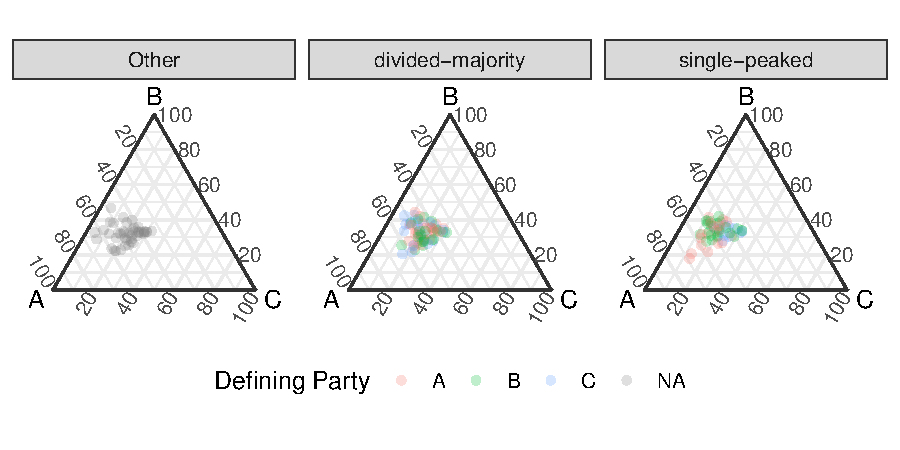
\includegraphics[width = \textwidth]{../output/figures/cses_fp.pdf}
	\caption{Distribution of first preferences in CSES cases, by class}
	\label{fig:cses_fp}
\end{figure}

The CSES dataset comprises a total of 162 cases, with a mean of 1384 and a standard deviation of 539 respondents per case.\footnote{Minimum: 360 respondents, Hong Kong 2004; maximum: 3795, New Zealand 1996.} Of these, we discarded two (Belarus 2008 and Lithuania 1997), because no respondent has complete preferences over all three parties. Figure~\ref{fig:case_map} Within each case, we applied the label $A$ to the party that most respondents stated as first preference; the label $B$ to the party that the second-most respondents stated as second preference; and, finally, the label $C$ to the party that the third-most respondents stated as their first preference. Thus, the expected ballot profile for all of the cases is $v_A > v_B > v_C$. 

\begin{figure}[!htb]
	\centering
	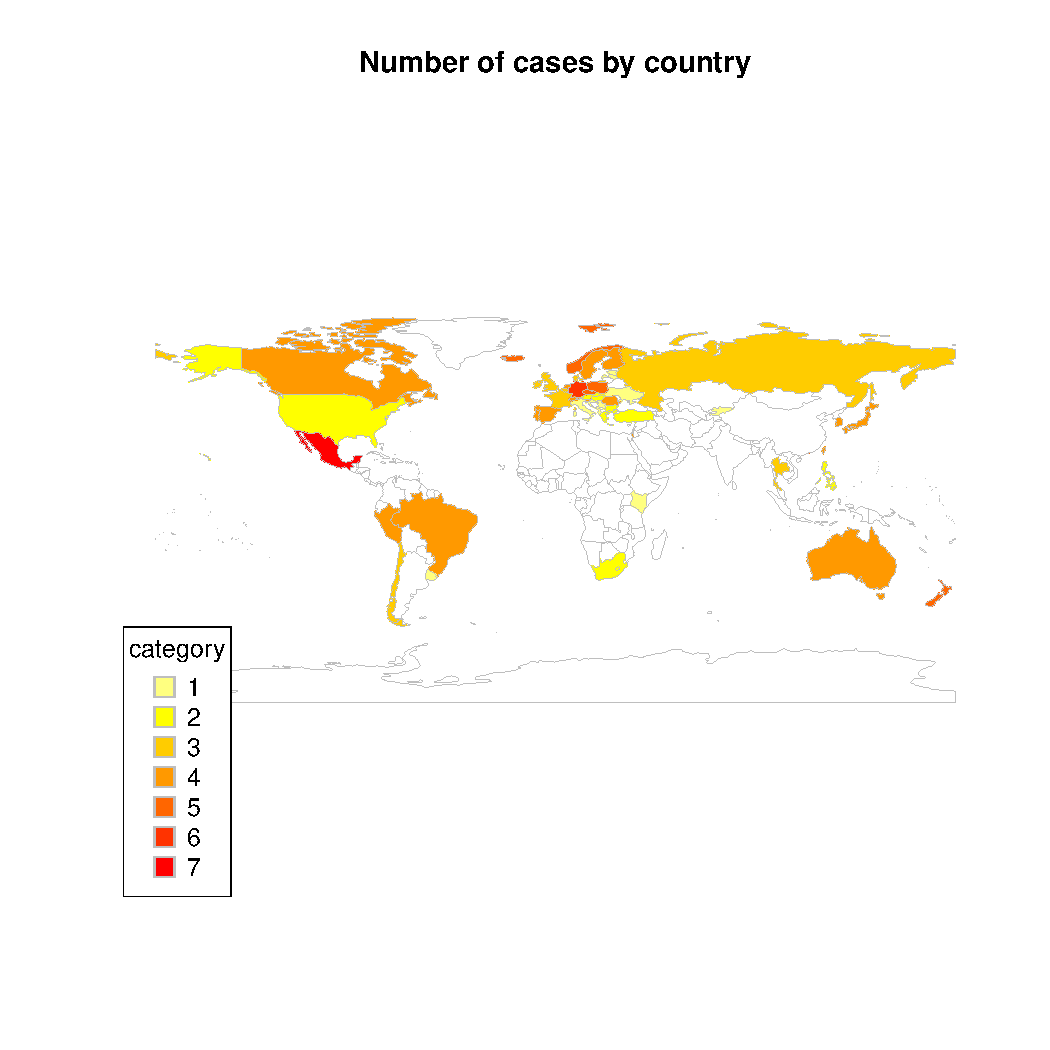
\includegraphics[width = .8 \textwidth]{../output/figures/case_map.pdf}
	\caption{Cases in CSES data, by country}
	\label{fig:case_map}
\end{figure}

\subsubsection{Characterising CSES cases}

How different are the CSES cases from one another? Putting the intensity of preferences aside, we can fully describe each case with the six-item vector $\bf v$. More intuitively, however, we can also describe the cases in terms of the distribution of first and second preferences.

\textbf{First preferences.} Figure~\ref{fig:cses_fp} plots the distribution of first preferences for each case on a ternary diagram. Given the above labelling convention, the distribution is tightly packed into one part of the simplex, its boundaries delineated by the $(1 - v_C) / 2$ boundary on the one side, and the $(1 - v_B) / 2$ on the other.\footnote{Conceptually, this makes sense: a violation of the first one would suggest that $v_B > v_A$, and a violation of the second one would suggest that $v_C > v_B$.} The figure groups together cases that share characteristics in second preferences (single-peaked, i.e. defining party is attractor; divided majority, i.e. defining party is repeller; and all others). There is no discernible difference in the distribution of first preferences between the groups; similarly, there is no discernible difference in the distribution conditional on the defining party. Note that even though the distribution is strongly centred on a particular part of the simplex, our labelling convention is without loss of generality: the results remain representative.

\textbf{Second preferences }Describing the distribution of second preferences, especially conditional on first preferences, once again would require the summary (or visualisation) of multidimensional relationships and an impractical number of permutations. (Note how an apt summary of this could be an entire new paper. Figure~\ref{fig:cses_fp} is probably the best we can do for now.)

We restrict our analysis of second preferences to two key points: First, preference distributions in the CSES can be broadly aligned along one dimension ranging from \emph{single-peaked} through \emph{neutral} to \emph{divided majority}. Second, we show how the CSES data is distributed along this spectrum.

The classification of cases has been briefly covered on page 17 in Andy's memo. For completeness' sake, let us state our approach again. Without loss of generality, call the candidate whose first-preference voters have the most equally split second preferences $X$, and the other two $Y$ and $Z$.\footnote{Technically, pick X such that $\mathrm{min} |m_j - 0.5|$.} If both $m_{YZ}, m_{ZY} > 0.6$, then classify this as a single-peaked case $X+$. Conversely, if both $m_{YZ}, m_{ZY} < 0.4$, then classify this as a divided-majority case $X-$. If $m_{YZ}, m_{ZY} \in [0.4, 0.6]$, then classify this as a neutral case, $N(A)$. If neither of these conditions hold (because of unusual second preferences), label this case as other ($O$). 

Table~\ref{tab:csesprefs} summarises the distribution of preference profiles found in the CSES data. Divided majority cases form the plurality of our dataset; however, there is also a large number of single-peaked cases. Fully neutral cases appear to be rarer. Out of the 160 cases in total, 27 cannot be classified using our approach and remain labelled as "other".\footnote{Do we need to show that our results do not depend on these cases?}

\begin{table}[tb]
	\caption{Distribution of preference profiles in CSES data}
	\label{tab:csesprefs}
	\centering

	\begin{tabular}{lccc}
	\hline

	\toprule
	\textbf{} & \textbf{A} & \textbf{B} & \textbf{C} \\
	\cmidrule{2-4}
	Single-peaked (+) & 18 & 23 & 9  \\
	Divided majority (-) & 28 & 20 & 20  \\
	Neutral () & 5 & 7 & 3  \\
	Other () & & 27 &  \\
	\bottomrule
	\end{tabular}
\end{table}

\subsection{Methods}

\todo[inline]{(So far, so good. We have described the data and justified the CSES.) Separate description of "methods" necessary?}

After calculating the strategic incentive for each voter in each case, and at different levels of $s$, we can perform further analyses to examine the three questions set out in the introduction of this section. First, we hold $s = 85$ constant and check to what extent strategic incentives by \emph{voter type} conform to the predictions made in the theoretical section. We do this by comparing conditional probabilities of strategic votes $YXZ$ and $ZXY$ being optimal for a $XYZ$ voter in each case in the CSES. Formally, we look at the distributions $\Prob(YXZ | XYZ \land C)$ and $\Prob(ZXY | XYZ \land C)$ where $C$ is one of the previously defined second-preference distribution classes ($A+$, $B+$, $\ldots$)

For comparing the extent and magnitude of incentives overall, we aggregate the proportions across both voter types and cases. Here, we are interested in the overall proportion of positive strategic incentives at different levels of information under both plurality and RCV. Furthermore, we also compare the proportion of voters with $\tau > 0$ under both RCV and plurality in each case, respectively. (\emph{What about interdependence?})

Finally, we perform analyses of overall performance of the two electoral systems. For each case, we calculate the probability of different voting paradoxes (non-monotonicity [RCV], no-show [RCV], [plurality]) to check which of the electoral systems is more vulnerable, given the empirical distribution of ballot profiles. We also check which of the two electoral systems is more likely to benefit the Condorcet winner, and how much of a difference strategic voting makes in terms of changing the winner (how?)

\section{Results: Strategic Voting by Second Preference Class}

Objective for this section: check whether theoretical predictions for different cases hold.

Expectation is that the empirics should broadly conform with our theory, but outliers / deviations will occur (for reasons that Andy described in the email).

\subsection{Single-Peaked}

\subsubsection{A is the attractor (A+)}

\begin{figure}[!htb]
	\centering
	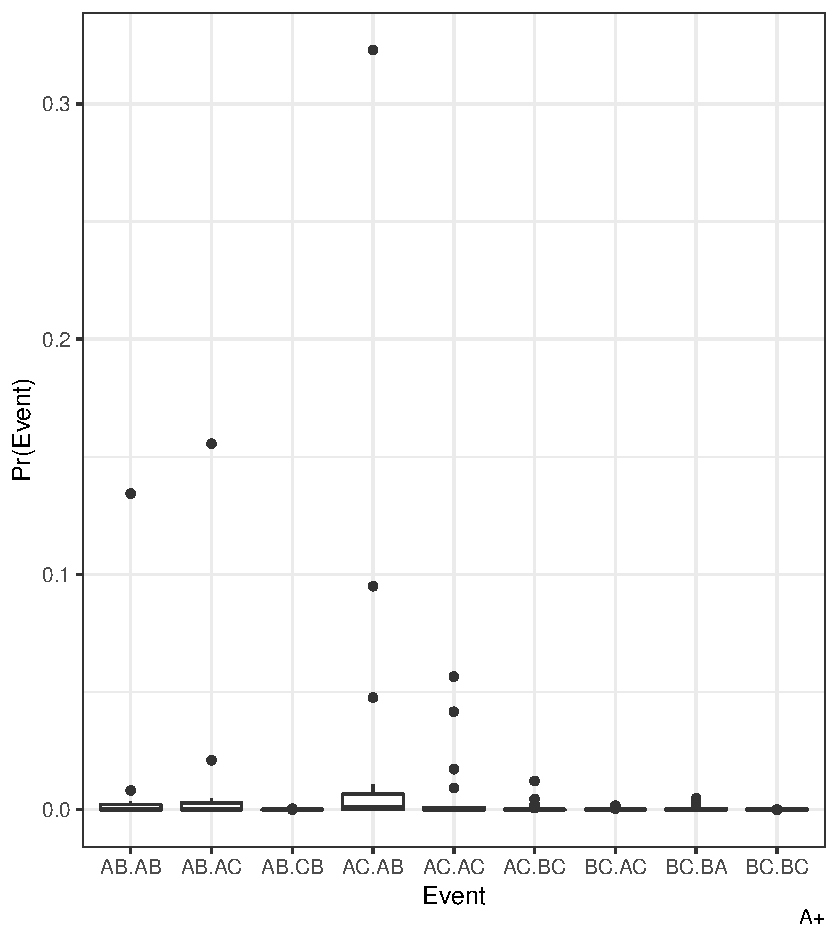
\includegraphics[width = .45\textwidth]{../output/figures/prediction/pprob_sp_a.pdf}
	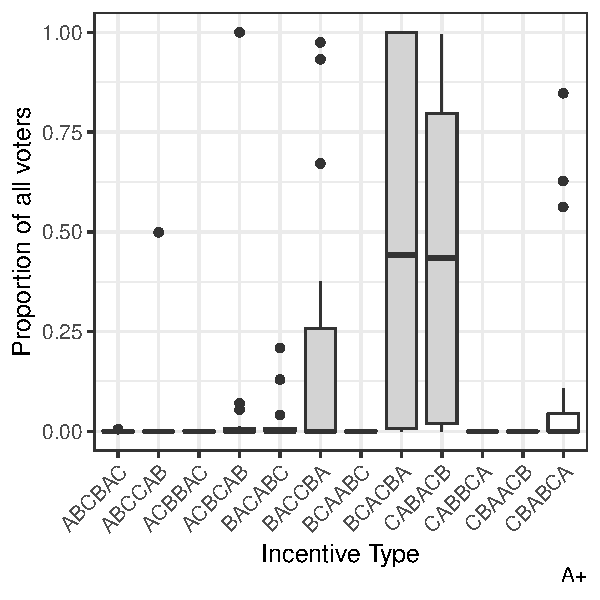
\includegraphics[width = .45\textwidth]{../output/figures/prediction/svinc_sp_a.pdf}
	\caption{Distribution of pivotal probabilities and proportions of strategic vote incentives for all $A+$ cases.}
	\label{fig:figure1}
\end{figure}

The theoretical prediction is that $AC.AB$ is the dominant pivotal event; this holds true in the empirical data. However, there are a few outliers with high probabilities for $AC.AC$ in particular, and a few for $AC.BC$. (Need to check whether $AB.XX$ events are non-trivial here). 

Consequently, the $CAB \rightarrow ACB$ strategic incentive is high. The $BCA \rightarrow CBA$ strategic incentive would only be attenuated by a high likelihood of $BC$ events in the second round; however, this does not seem to be the case and thus the $BCA \rightarrow CBA$ incentive is also very strong. Finally, the $BAC \rightarrow CBA$ incentive is attenuated by both $BC$ \textit{and} $AC$ and occurs much rarer. Note that the mean levels of strategic incentive proportions for $CAB \rightarrow ACB$ and $BCA \rightarrow CBA$ are much lower than for the $B+$ and $C+$ cases -- this is because, in relative terms, the $AC.AB$ event is much less likely than the $BC.XX$ ones.

\subsubsection{B is the attractor (B+)}

This is the old case of B having neutral preferences and A, C voters both choosing B in second preferences.

\begin{figure}[!htb]
	\centering
	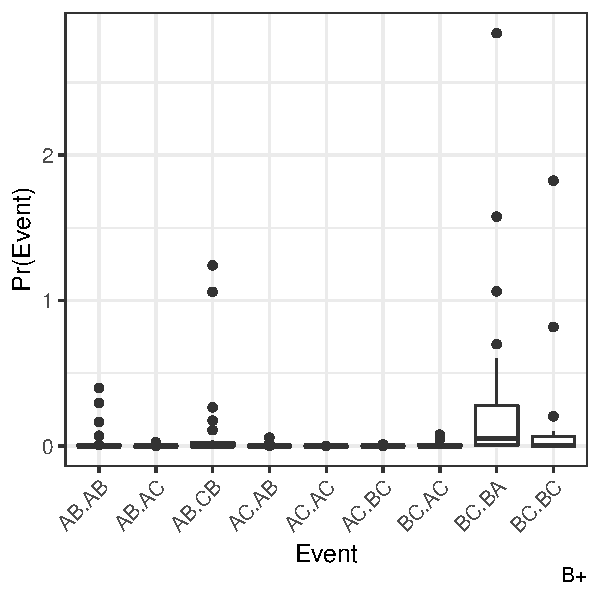
\includegraphics[width = .45\textwidth]{../output/figures/prediction/pprob_sp_b.pdf}
	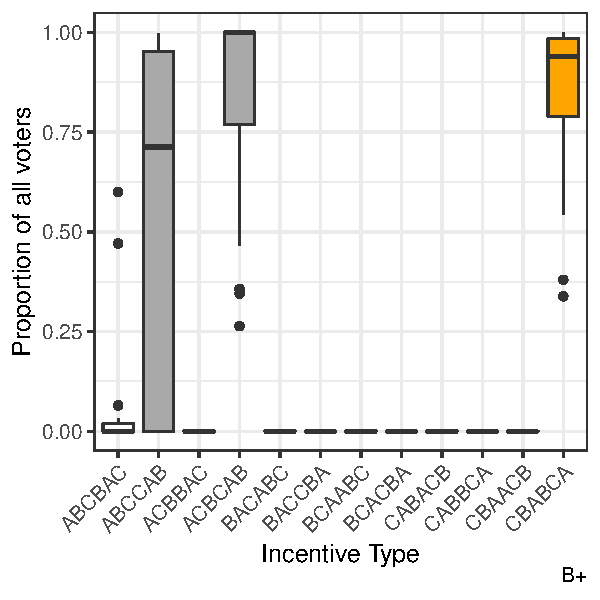
\includegraphics[width = .45\textwidth]{../output/figures/prediction/svinc_sp_b.pdf}
	\caption{Distribution of pivotal probabilities and proportions of strategic vote incentives for all $B+$ cases.}
	\label{fig:figure1}
\end{figure}

As predicted by the theory, the $BC.BA$ pivotal event clearly dominates here, with $BC.BC$ coming second.

Unsurprisingly, this means that the incentive to vote $CBA \rightarrow BCA$ is very high -- in only two cases have less than half of all $CBA$ voters an incentive to follow this insincere vote. However, the proportion of $ACB \rightarrow CAB$ incentives is also very high (in fact, the mean is even higher!). This is because the likelihood of a conflicting $AC$ event in the second round is extremely small (given our labelling of the parties). Graphically, it seems that the majority of our $B+$ cases also have $B$'s second preferences slightly tilt to the right, which (I think) decreases the probability of this vote type "backfiring". Finally, the $ABC \rightarrow CAB$ incentive is, again, somewhat lower, and experiences a lot more variance than the others, because of the additional consideration of the (more likely) $BC$ second-round event. 

Here, the prediction for the crossed out elements does not appear to hold, because in the empirics, the second-round pivotal events appear to be much less likely.

\subsubsection{C is the attractor (C+)}

\begin{figure}[!htb]
	\centering
	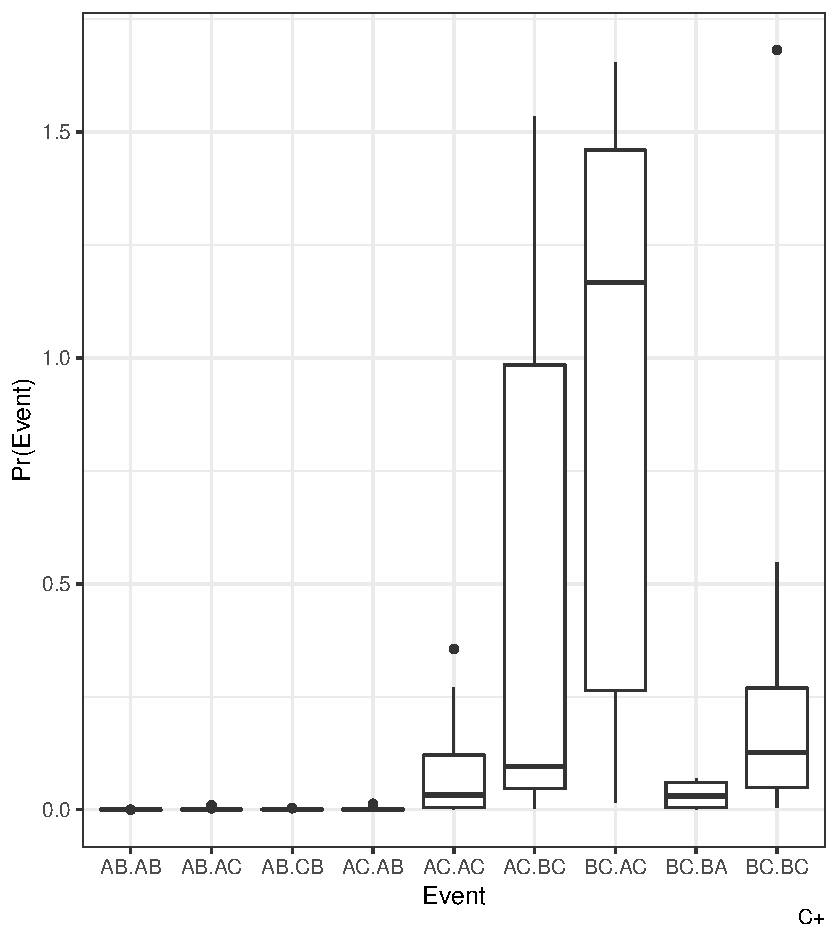
\includegraphics[width = .45\textwidth]{../output/figures/prediction/pprob_sp_c.pdf}
	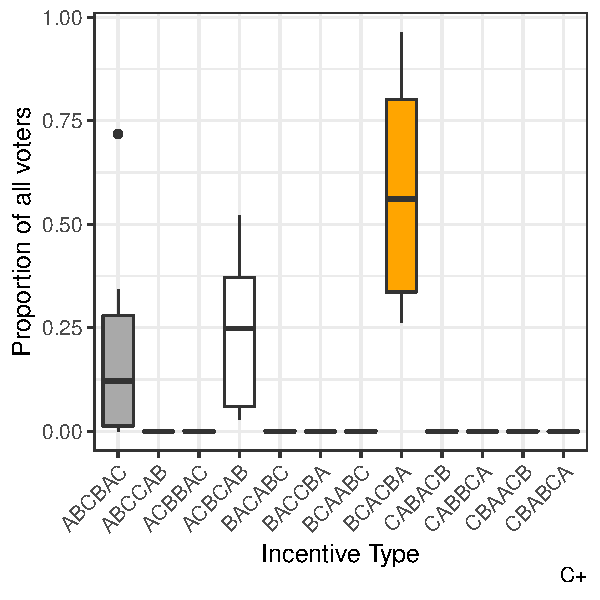
\includegraphics[width = .45\textwidth]{../output/figures/prediction/svinc_sp_c.pdf}
	\caption{Distribution of pivotal probabilities and proportions of strategic vote incentives for all $C+$ cases.}
	\label{fig:figure1}
\end{figure}

Here, the $BC.AC$ event is clearly the dominant one, however, we see a few others ($AC.AC$, $AC.BC$, $BC.BC$) that are also relevant. Consequently, because of the high $BC.AC$ probability, the predicted $BCA \rightarrow CBA$ incentive is also the most prevalent one. There is also some incidence of the $ABC \rightarrow BAC$ incentive, which would only be mitigated by the $AB$ second-round pivotal event (which is quite likely, no?). Surprisingly, $ACB$ voters appear to have some incentive to vote $\rightarrow CAB$. This is probably because of the high probablity of $AC.BC$: here, a sincere vote would help elect the least preferred candidate (no-show). Thus, if C is the attractor, the predictions don't hold as well.

\begin{figure}[!htb]
	\centering
	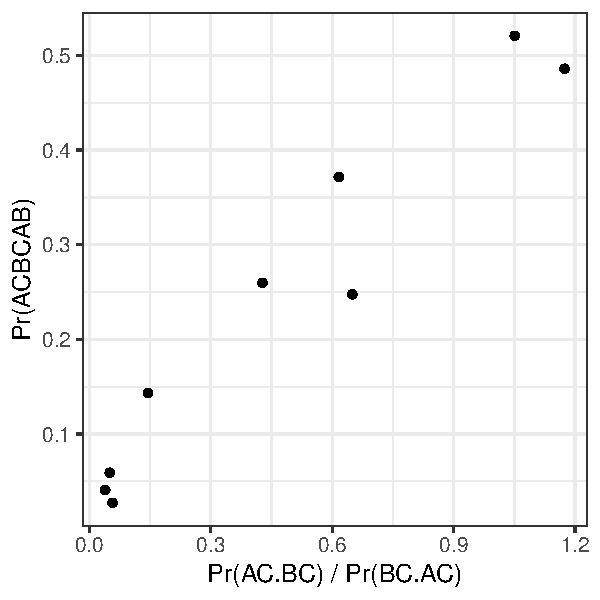
\includegraphics[width = .45\textwidth]{../output/figures/prediction/sp_c_odd.pdf}
	\caption{Proportion of $ACB$ voters with incentive to vote $CAB$ by the probability of the $AC.BC$ pivotal event relative to $BC.AC$.}
	\label{fig:figure1}
\end{figure}

\subsection{Divided Majority}

\subsubsection{A is the repeller (A-)}

\begin{figure}[!htb]
	\centering
	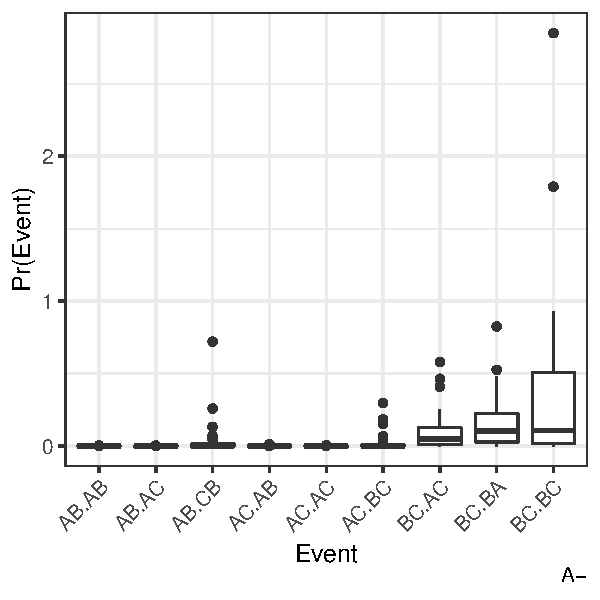
\includegraphics[width = .45\textwidth]{../output/figures/prediction/pprob_dm_a.pdf}
	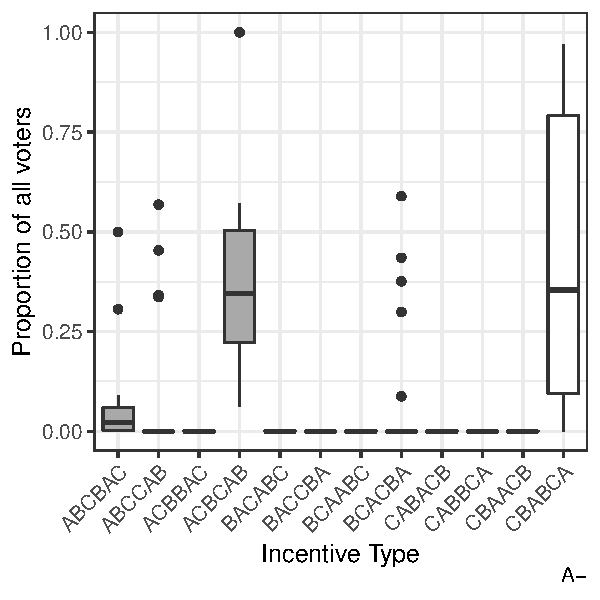
\includegraphics[width = .45\textwidth]{../output/figures/prediction/svinc_dm_a.pdf}
	\caption{Distribution of pivotal probabilities and proportions of strategic vote incentives for all $A-$ cases.}
	\label{fig:figure1}
\end{figure}

In the cases where $A$ is the repeller, we expect $BC.BC$ to be the dominant first-round pivotal event. This is, indeed, the case; however, on average, the $BC.BA$ event is just as likely. The predicted strategic incentives only affect a fraction of the potential voters. The $ABC \rightarrow BAC$ incentive is virtually non-existent while the $ACB \rightarrow CAB$ incentive affects a sizeable minority on average. The $CBA \rightarrow BCA$ incentive is unexpected and shows up with a lot of variance across the cases: some cases see almost all $CBA$ voters have this incentive whilst others barely feature it at all. (What explains it?)

\subsubsection{B is the repeller (B-)}

\begin{figure}[!htb]
	\centering
	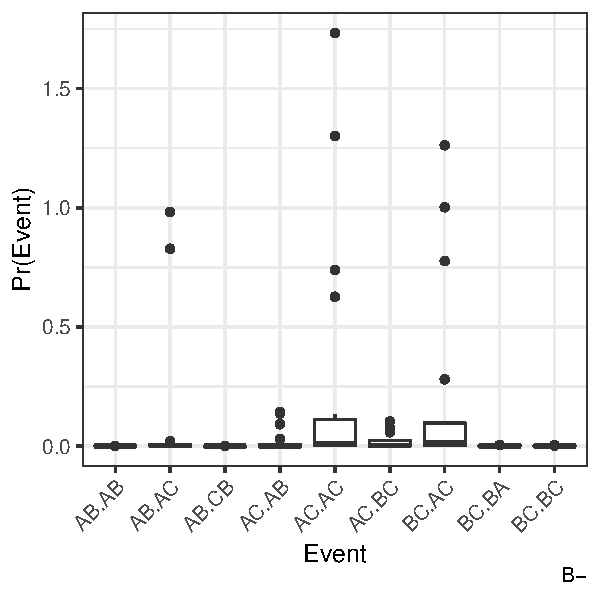
\includegraphics[width = .45\textwidth]{../output/figures/prediction/pprob_dm_b.pdf}
	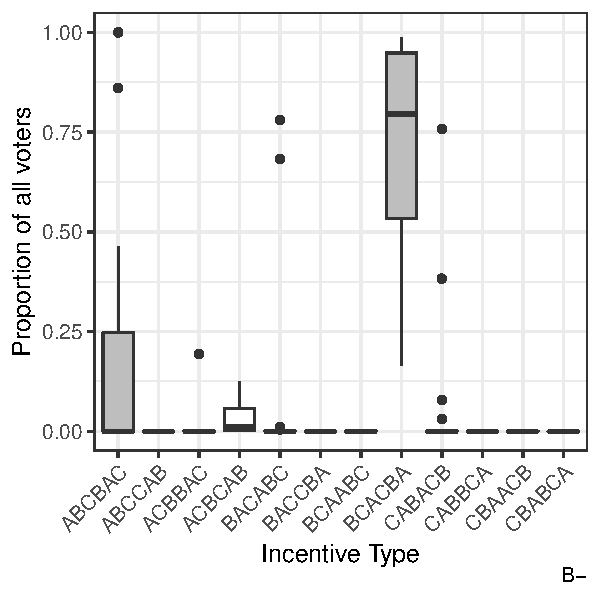
\includegraphics[width = .45\textwidth]{../output/figures/prediction/svinc_dm_b.pdf}
	\caption{Distribution of pivotal probabilities and proportions of strategic vote incentives for all $B-$ cases.}
	\label{fig:figure1}
\end{figure}

In the cases where $B$ is the repeller, we would expect $BC.AC$ to be the dominant pivotal event. Empirically, it is jointly dominant along with $AC.AC$ (at least in the aggregate). Because of that, the $ABC \rightarrow BAC$ incentive is diminished, while the predicted $BCA \rightarrow CBA$ incentive is very strong. Across the board, there are few other incentives.

\subsubsection{C is the repeller (C-)}

Where $C$ is the repeller, we would expect $BC.BA$ to be the dominant pivotal event. This may be true here, but the pivotal probabilities are very small for all types, with a few extreme outliers that may be driving the results here.

In terms of strategic incentives, we do observe the predicted $CBA \rightarrow BCA$ very strongly; the other two ($ABC \rightarrow CAB$ and $ACB \rightarrow CAB$) also feature, although with more variance. This is expected, as these depend more on the pivotal probability of $BC.BA$, which, as just explained, is not always dominant. (There is also the possibility that the variance is caused by underlying variance in the second-round $AC$ pivotal probability.)

\begin{figure}[!htb]
	\centering
	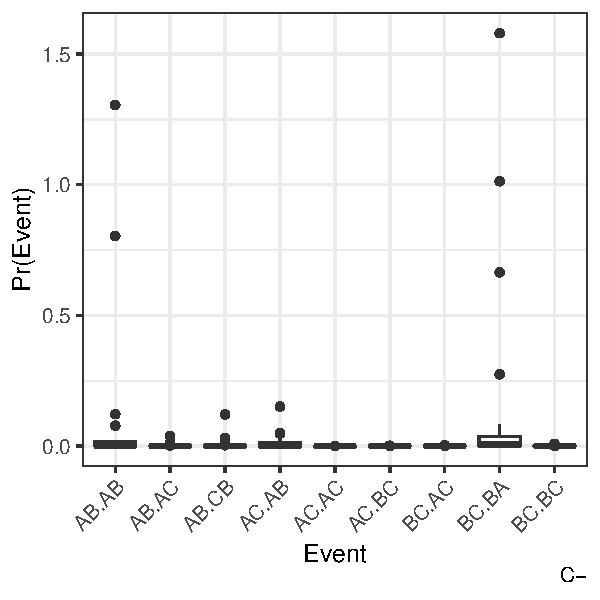
\includegraphics[width = .45\textwidth]{../output/figures/prediction/pprob_dm_c.pdf}
	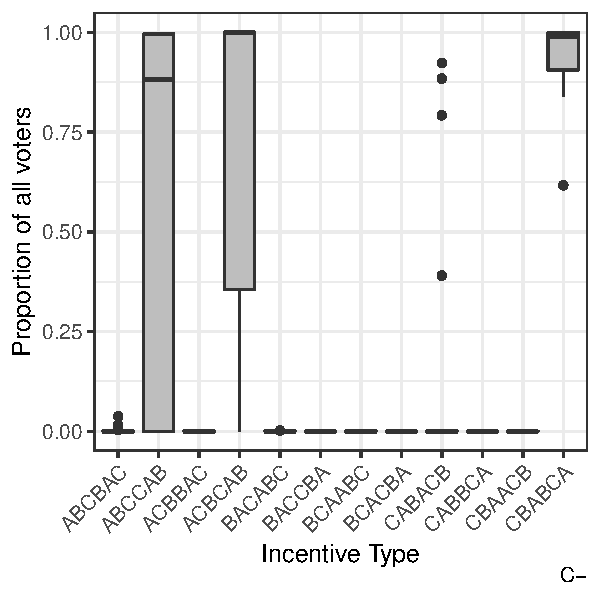
\includegraphics[width = .45\textwidth]{../output/figures/prediction/svinc_dm_c.pdf}
	\caption{Distribution of pivotal probabilities and proportions of strategic vote incentives for all $C-$ cases.}
	\label{fig:figure1}
\end{figure}


\section{Results: Incentives}

Next, we want to see what the distribution of likely voter preferences and ballot profiles means for the resulting strategic incentives, and differences between RCV and plurality. In Figure~\ref{fig:sv_prop}, each thin line describes the proportion of respondents with a positive strategic incentive for a given ballot, within a CSES case, at different levels of information.\footnote{Note that the existence of positive strategic incentives is non-exclusive; a voter may have a positive incentive to put both their second and their third preference first. The optimal ballot ordering will be the one for which the strategic incentive is greatest. (Need to check how code handles these situations.)}

\begin{figure}[!h]
	\centering
	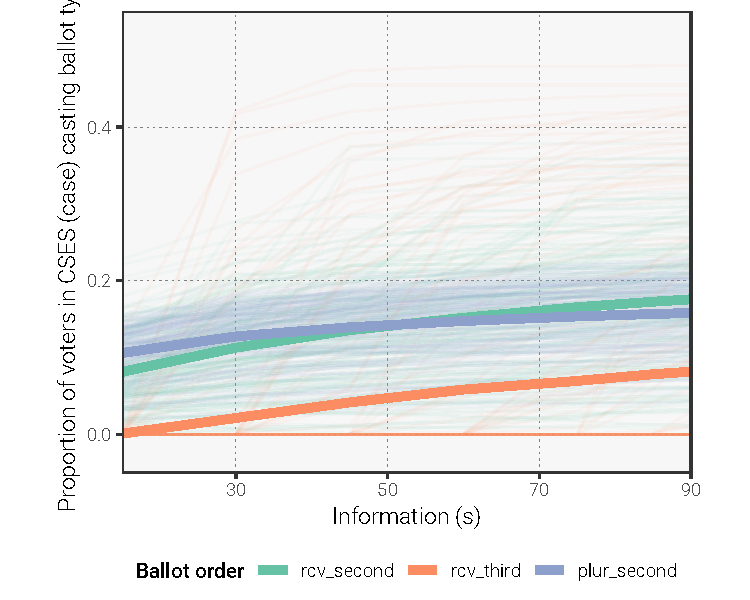
\includegraphics[width = .6 \textwidth]{../output/figures/cses_freq.pdf}
	\caption{Proportion of voters with non-sincere optimal vote, by level of information. Left panel: NSW. Right panel: CSES}
	\label{fig:sv_prop}
\end{figure}

Under plurality, there exists only one possible optimal strategic vote: to vote for one's second preference instead in order to avoid a wasted vote. This is only reasonable when one expects one's first preference to come last. In the CSES data, we observe the proportion of voters with a positive strategic incentive under Plurality to be capped at around 20 per cent. The incentive is also hardly sensitive to levels of information, suggesting that, overall, there is a relatively robust set of voters with a strategic incentive that requires very little information altogether under plurality.

Under RCV, this is a little bit different. We note that the incentive to rank one's second preference first behaves somewhat similar to the strategic incentive under Plurality. However, it is a little bit more sensitive to the levels of information (rising from about 0.1 at $s = 15$ to 0.2 at $s = 90$); furthermore, the variance across cases is also higher. Finally, the incentive to rank one's third preference first increases rapidly as information improves. This type of incentive is motivated by a strong pushover; with better information, the probablity of accidentally electing one's most-disliked choice into office diminishes (This already hints at a coordination problem under RCV.)

Taking the strategic incentives for second and third together, this supports our theoretical prediction that the incidence of positive strategic incentives under RCV is higher than under Plurality (that is, at realistic (?) levels of information).

\subsection{Direct Comparison of Frequency}

So far, we have been dealing with aggregates. How does the difference between RCV and Plurality play out in each individual case? To examine this, we took the overall proportion of voters with a positive strategic incentive under either system and plotted them against each other in Figure~\ref{fig:sv_dist}. Cases below the 45 degree line have more voters with a positive strategic incentive under plurality; cases above the 45 degree line have more voters with a positive strategic incentive under RCV.

\begin{figure}[!h]
	\centering
	\includegraphics[width = .6 \textwidth]{"../output/figures/cses_prop"}
	\caption{Proportion of voters with non-sincere optimal vote, by level of information. Left panel: NSW. Right panel: CSES}
	\label{fig:sv_dist}
\end{figure}

At low levels of information ($s = 15$), the cases are clustered fairly equally around either side of the 45 degree line. However, as beliefs become more precise, strategic votes become much more common under RCV, whilst the proportion under plurality remains capped at around 0.2. We note that there is a substantial proportion of cases that remain below the 45 degree line, even with very precise beliefs. This underlines the importance of empirical results: it is entirely possible to come up with all kinds of theoretical cases that yield different results. With the CSES data, we get a sense of likely preference distributions and ballot profiles, and can thus present results that are more likely to hold in real elections. In this case, while there are a few cases where the proportion of voters with a positive strategic incentive is greater under Plurality, in the majority of cases, RCV offers greater strategic incentives (see Table~\ref{tab:strat_inc}).

Figure~\ref{fig:sv_dist} plots the proportion of "optimal" strategic voters under RCV and Plurality for each case seperately. This further supports the conclusions from the previous section: For the most part, the proportion of strategic voters under plurality remains capped at around $\approx 0.2$. For low levels of $s$, the cases are distributed around very low levels of strategic voting under both electoral systems. However, as information increases, the proportion of voters with a positive incentive under AV increases dramatically.

\begin{table}[!htb]
	\caption{Number of cases where RCV incentive is greater}
	\label{tab:strat_inc}
	\centering

	\begin{tabular}{lccc}
	\toprule
	s & \textbf{RCV $>$ Plur} & \textbf{RCV $<$ Plur} & \textbf{Proportion RCV} \\
	\cmidrule{2-4}
	15 & 41 & 119 & 0.256 \\
	30 & 58 & 102 & 0.362 \\
	45 & 66 & 94 & 0.412 \\
	60 & 73 & 87 & 0.456 \\
	75 & 83 & 77 & 0.519 \\
	85 & 88 & 72 & 0.550 \\
	90 & 90 & 70 & 0.563 \\
	\bottomrule
	\end{tabular}
\end{table}

Why, then, is this not something that political debates about RCV have picked up so far? (1) So far, we don't know how large that incentive to vote strategically is. It may be extremely small, and, assuming costs to strategic voting, ultimately not worth it. (2) Parties may have incorporated such strategic considerations in their how-to-vote cards, thus reducing costs for voters. (Can we check this empirically?)

\subsection{QQ-Plots}

\begin{figure}[!h]
	\centering
	\includegraphics[width = .6 \textwidth]{"../output/figures/cses_qq"}
	\caption{QQ-Plot of strategic incentives, $\tau$, under Plurality (x) and RCV (y). Left panel: NSW. Right panel: CSES.}
	\label{fig:qqplots}
\end{figure}

So far, we have shown the following: (1) We can classify most empirical cases into two main categories, and predict fairly well what kind of strategic incentives exist. (2) The incidence of positive strategic incentives is somewhat greater under RCV than it is under Plurality. (Elaborate why this is important to show empirically, not just theoretically). But exactly how large are these incentives: do they warrant acting upon? Fortunately, our approach of calculating pivotal probabilities and expected utilities allows us to quantify the magnitude of the strategic incentive ($\tau$, see also Eggers and Vivyan 2018). 

Figure~\ref{fig:qqplots} compares the distribution of strategic incentives under both plurality and RCV, conditional on $s$, in QQ-Plots. 

(Explain how these plots work and how to interpret them. Not all readers may be familiar with them.)

A couple of general observations: (1) The greater $s$, the greater the variance in both $\tau_{RCV}$ and  $\tau_{P}$. This makes sense: when I know very little about the likely electoral outcome, voting sincerely is a less risky strategy, and incentives to vote strategically are smaller. (2) For any level of $s$, \textit{negative} strategic incentives (i.e., situations where the sincere vote is the optimal vote) are relatively more common. (3) Conversely, for any level of $s$, (small and moderate) \textit{positive} strategic incentives are more common under plurality. This is not true of very high levels of $\tau$, which are, again, more common under RCV (see how the aggregate line crosses the 45-degree line in the CSES panel again). (4) The Australian case features smaller incentives to vote strategically overall (?) -- this may have to do with the relative weakness of the Greens. 

The main takeaway here is that strategic voting under RCV, for the most part, brings smaller benefits compared to a sincere vote. There are, however, a few situations at the extreme end where there is a very high incentive under RCV.

What this means is that if we assume strategic voting to be costly (relative to a sincere vote), then we would observe much less of it in RCV. This is equivalent to calculating $\hat{\tau} \equiv \tau - c$, where $c$ is a constant cost. Under RCV, this would shift a much greater part of the distribution into the negative domain, thus attenuating any strategic incentive.

\section{Results: Electoral System Performance}
\subsection{Incidence of Voting Paradoxes}

\begin{figure}[!h]
	\centering
	\includegraphics[width = .6 \textwidth]{"../output/figures/paradoxes_cses"}
	\caption{Probability of voting paradoxes under RCV over probability of wasted vote under plurality. Left panel: NSW. Right panel: CSES}
	\label{fig:paradox}
\end{figure}

Figure~\ref{fig:paradox} plots the probability of different voting paradoxes under RCV over the probability of wasting one's vote under plurality. This is conditional on $s = 85$. In both cases, there is a higher chance of the non-monotonicity paradox occuring than there is of the the no-show paradox occuring. However, in either situation this is overshadowed by the much higher probablity of casting a wasted vote under plurality: the entire sample fits to the right of the 45-degree line. What this suggests is that, no matter what the strategic voting incentives, RCV is much better at avoiding tricky electoral situations.

\textit{(Need to check why in the Australian case Pr(Wasted Vote) begins at $\approx 0.2$)}

Also note that the LOESS in the Australian case probably suffers from overfitting - one or two observations towards the high end of Pr(Wasted Vote) pull the non-mon curve downwards.

\subsection{Interdependence} \label{interdep}

\begin{figure}[!h]
	\centering
	\includegraphics[width = .6 \textwidth]{"../output/figures/cses_l0"}
	\caption{Proportion of voters whose Level-2 strategic vote differs from their sincere vote, conditional on proportion of Level 2 strategic voters in population ($\lambda$). Left panel: NSW. Right panel: CSES.}
	\label{fig:figure1}
\end{figure}

\begin{figure}[!h]
	\centering
	\includegraphics[width = .6 \textwidth]{"../output/figures/cses_l1"}
	\caption{Proportion of voters whose Level-2 strategic vote differs from their Level-1 strategic vote, conditional on proportion of Level 2 strategic voters in population ($\lambda$). Left panel: NSW. Right panel: CSES.}
	\label{fig:figure1}
\end{figure}

Need to provide interpretation still.

\subsection{Condorcet Winner}

\section{Conclusion}

\end{document}